\section{Examples}
\begin{example}
(Dido's problem / Isoperimetric problem)\\
The task is to maximize the area enclosed by a curve of prescribed length. More precisely, an interval $[a,b]\subset\mathbb{R}$ is given and we consider functions $u:[a,b]\longrightarrow\mathbb{R}$ which have length $L_0>0$. We search for some function $u_*:[a,b]\longrightarrow\mathbb{R}$ such that the area under this curve is maximal. See \hyperref[fig:example_1_2_1]{Figure I.1} for an illustration. Mathematically, this can be formulated as follows: Find $u\in C_0^1([a,b])=\{u\in C^1([a,b])\mid u(a)=u(b)=0\}$ such that the parameter
\[L(u)=\int_a^b{\sqrt{1+(u'(x))^2}\mathrm{d}x}=L_0>0\]
is fixed, and the area
\[I(u)=\int_a^b{u(x)\mathrm{d}x}\]
is maximal. This fits into our general setting we have described in the previous section by looking at $-I$ instead of $I$.\\[11pt]

\begin{figure}
	\centering
	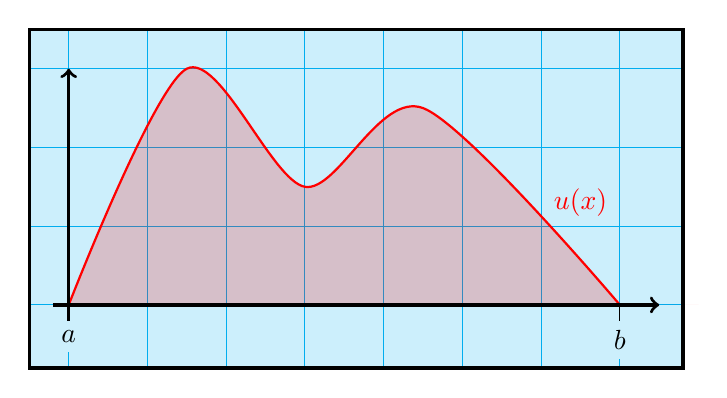
\begin{tikzpicture}
		% Hintergrund
		\fill[cyan!20] (-0.5, -0.8) rectangle (7.8, 3.5);
		\draw[thin, cyan] (-0.5, -0.8) grid (7.8, 3.5);

		% Funktion
		\fill[red, opacity=0.2] (8, 0) -- (0, 0) plot[smooth] coordinates {(0, 0) (1.5, 3) (3, 1.5) (4.5, 2.5) (7, 0)};
		\draw[thick, red] plot[smooth] coordinates {(0, 0) (1.5, 3) (3, 1.5) (4.5, 2.5) (7, 0)};
		\node[red] at (6.5, 1.3) {$u(x)$};

		% Achsen
		\draw[very thick, ->] (-0.2, 0) -- (7.5, 0);
		\draw[very thick, ->] (0, -0.2) -- (0, 3);
		\draw[thin] (0, 0) -- (0, -0.2) node[fill=cyan!20, below] {$a$};
		\draw[thin] (7, 0) -- (7, -0.2) node[fill=cyan!20, below] {$b$};

		% Rahmen
		\draw[very thick] (-0.5, -0.8) rectangle (7.8, 3.5);
	\end{tikzpicture}
	\caption{Example of a curve for Dido's problem.}
	\label{fig:example_1_2_1}
\end{figure}
\end{example}

\begin{example}
(Brachistochrone problem / Shortest time problem)\\
This was studied mathematically first by \textsc{Johann Bernoulli} in 1696. This was the example where calculus of variations more or less was invented. As in \hyperref[fig:example_1_2_2]{Figure I.2} illustrated, a mass $m>0$ is given and it should slide from point $(a,A)$ to $(b,B)$ under the influence of gravity.\\

\begin{figure}[ht]
	\centering
	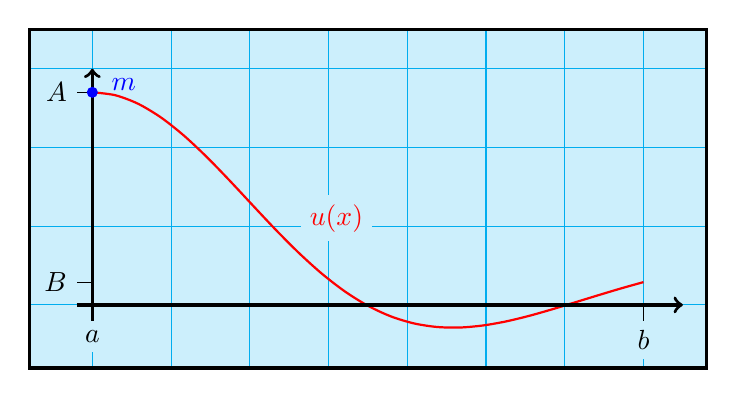
\begin{tikzpicture}
		% Hintergrund
		\fill[cyan!20] (-0.8, -0.8) rectangle (7.8, 3.5);
		\draw[thin, cyan] (-0.8, -0.8) grid (7.8, 3.5);

		% Funktion
		\node[red, fill=cyan!20] at (3.1, 1.1) {$u(x)$};
		\draw[thick, red] plot[smooth, domain=0:7] (\x, {0.7+(2-0.3*(\x)^2)*exp(-0.07*(\x)^2)});

		% Achsen
		\draw[very thick, ->] (-0.2, 0) -- (7.5, 0);
		\draw[very thick, ->] (0, -0.2) -- (0, 3);
		\draw[thin] (0, 2.7) -- (-0.2, 2.7) node[fill=cyan!20, left] {$A$};
		\draw[thin] (0, 0.2887) -- (-0.2, 0.2887) node[fill=cyan!20, left] {$B$};
		\draw[thin] (0, 0) -- (0, -0.2) node[fill=cyan!20, below] {$a$};
		\draw[thin] (7, 0) -- (7, -0.2) node[fill=cyan!20, below] {$b$};
		\fill[blue] (0, 2.7) circle (2pt);
		\node[blue] at (0.4, 2.8) {$m$};

		% Rahmen
		\draw[very thick] (-0.8, -0.8) rectangle (7.8, 3.5);
	\end{tikzpicture}
	\caption{Example of a slide.}
	\label{fig:example_1_2_2}
\end{figure}

The question is how to build the slide such that the time on the slide is short. We need some physical laws to derive our formulas. Let $u:[a,b]\longrightarrow\mathbb{R}$ be the function describing our slide. At $x\in[a,b]$ the position is given by $p(x)=\begin{pmatrix}x\\u(x)\end{pmatrix}$ and the velocity at position $p$ is
\[v(x)=\frac{\mathrm{d}}{\mathrm{d}t}p(x)=\begin{pmatrix}\dot x\\u'(x)\cdot\dot x\end{pmatrix},\]
where $\dot x=\frac{\mathrm{d}}{\mathrm{d}t}x$. The kinetic and potential energy of the mass is given by
\begin{align*}
	E_{\text{kin}}&=\frac{1}{2}\cdot m\cdot\lvert v\rvert^2=\frac{1}{2}\cdot m\cdot\dot x^2\cdot(1+(u'(x))^2),\\
	E_{\text{pot}}&=m\cdot g\cdot h=m\cdot g\cdot u(x),
\end{align*}
where $g$ denotes the gravitational acceleration. Both energies are transformed into each other, i.e. they are conserved. This means it holds
\[m\cdot g\cdot A=m\cdot g\cdot u(0)=m\cdot g\cdot u(x)+\frac{1}{2}\cdot m\cdot\dot x^2\cdot(1+(u'(x))^2).\]
After simplification and rearranging terms we obtain
\[\dot x^2=\frac{2g(A-u(x))}{1+(u'(x))^2}.\]
From this formula we can derive the sliding time. Via separation of variables we obtain
\[T(u)=\int_0^{T(u)}{1\mathrm{d}t}=\int_{x(0)}^{x(T(u))}{\frac{1}{\dot x}\mathrm{d}x}=\int_a^b{\sqrt{\frac{1+(u'(x))^2}{2g(A-u(x))}}\mathrm{d}x}.\]
The task now is to find a $C^1$-function $u$ with $u(a)=A$ and $u(b)=B$ such that $T(u)$ is minimal. This problem also falls into our class. Until now, we cannot solve this. The solution is given by a cycloid.
\begin{figure}[ht]
	\centering
	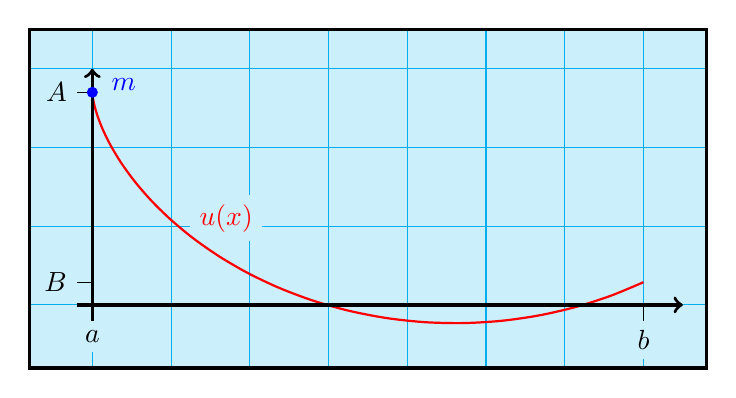
\begin{tikzpicture}
		% Hintergrund
		\fill[cyan!20] (-0.8, -0.8) rectangle (7.8, 3.5);
		\draw[thin, cyan] (-0.8, -0.8) grid (7.8, 3.5);

		% Funktion
		\node[red, fill=cyan!20] at (1.7, 1.1) {$u(x)$};
		\draw[thick, red] plot[smooth, domain=0:4.01133] ({1.46582*(\x-sin(180*\x/pi))}, {1.46582*(cos(180*\x/pi)-1)+2.7});

		% Achsen
		\draw[very thick, ->] (-0.2, 0) -- (7.5, 0);
		\draw[very thick, ->] (0, -0.2) -- (0, 3);
		\draw[thin] (0, 2.7) -- (-0.2, 2.7) node[fill=cyan!20, left] {$A$};
		\draw[thin] (0, 0.2887) -- (-0.2, 0.2887) node[fill=cyan!20, left] {$B$};
		\draw[thin] (0, 0) -- (0, -0.2) node[fill=cyan!20, below] {$a$};
		\draw[thin] (7, 0) -- (7, -0.2) node[fill=cyan!20, below] {$b$};
		\fill[blue] (0, 2.7) circle (2pt);
		\node[blue] at (0.4, 2.8) {$m$};

		% Rahmen
		\draw[very thick] (-0.8, -0.8) rectangle (7.8, 3.5);
	\end{tikzpicture}
	\caption{Solution of Brachistochrone problem.}
\end{figure}\\
\end{example}
\begin{example}
(Minimal surface / Shape of a soap film)
\begin{itemize}
	\item[(a)] Let $\Omega\subset\mathbb{R}^2$ and $g\in C^0(\partial\Omega)$ be given. Find $u\in C^0(\overline{\Omega})\cap C^1(\Omega)$ that minimizes the area
	\[I(u)=\int_\Omega{\sqrt{1+\lvert\nabla u(x)\rvert^2}\mathrm{d}x}\]
	and satisfies $u|_{\partial\Omega}=g$. This problem is illustrated in \hyperref[fig:example_1_2_3_a]{Figure I.4}.

	\begin{figure}[ht]
		\centering
		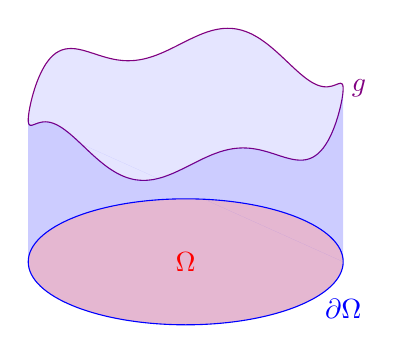
\begin{tikzpicture}
			% Ellipse
			\filldraw[fill=red, fill opacity=0.2, draw=blue] ellipse (2 and 0.8);

			% Funktion
			\filldraw[fill=blue, fill opacity=0.1, draw=violet] plot[smooth, domain=0:360, samples=100] ({2*cos(\x)}, {2+0.2*cos(5*\x)+0.8*sin(\x)});

			\fill[blue, opacity=0.1] ellipse (2 and 0.8);
			\fill[blue, opacity=0.2] (2, 0) arc (0:180:2 and 0.8) -- (-2, 1.8) plot[smooth, domain=180:360] ({2*cos(\x)}, {2+0.2*cos(5*\x)+0.8*sin(\x)}) -- (2, 0);

			% Beschriftungen
			\node[red] at (0, 0) {$\Omega$};
			\node[blue] at (2, -0.6) {$\partial\Omega$};
			\node[violet] at (2.2, 2.2) {$g$};
		\end{tikzpicture}
		\caption{Setting of minimal surface problem.}
		\label{fig:example_1_2_3_a}
	\end{figure}
	\item[(b)] There is a variant of the problem. Let $R_0,R_L>0$ be given. The goal is to find a minimal surface of the revolution.\\

	\begin{center}
		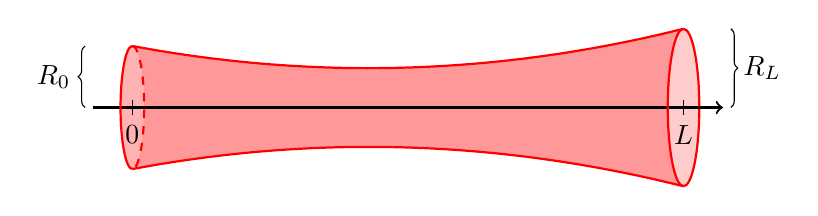
\begin{tikzpicture}
			% Rotationsvolumen Flächen einfärben
			\fill[red, opacity=0.2] (7, 0) ellipse (0.2 and 1);
			\fill[red, opacity=0.3] (0, 0) ellipse (0.15 and 0.78125);
			\fill[red, opacity=0.4] plot[smooth, domain=0:7] (\x, {(\x-3)^2/32+0.5}) arc (90:270:0.2 and 1) plot[smooth, domain=7:0] (\x, {-(\x-3)^2/32-0.5}) arc (-90:90:0.15 and 0.78125);

			% Rotationsvolumen Linien
			\draw[thick, red] plot[smooth, domain=0:7] (\x, {(\x-3)^2/32+0.5});
			\draw[thick, red] plot[smooth, domain=0:7] (\x, {-(\x-3)^2/32-0.5});
			\draw[thick, red] (7, 1) arc (90:-90:0.2 and 1);
			\draw[thick, red, dashed] (0, 0.78125) arc (90:-90:0.15 and 0.78125);

			% Achse und Radien benennen
			\draw[thick, ->] (-0.5, 0) -- (7.5, 0);
			\draw[thin] (0, 0.1) -- (0, -0.1) node[below] {0};
			\draw[thin] (7, 0.1) -- (7, -0.1) node[below] {$L$};
			\draw[decorate,decoration={brace}] (-0.6, 0) -- (-0.6, 0.78125);
			\node at (-1, 0.39) {$R_0$};
			\draw[decorate,decoration={brace}] (7.6, 1) -- (7.6, 0);
			\node at (8, 0.5) {$R_L$};

			% Rotationsvolumen elliptische Linien im Vordergrund
			\draw[thick, red] (7, 1) arc (90:270:0.2 and 1);
			\draw[thick, red] (0, 0.78125) arc (90:270:0.15 and 0.78125);
		\end{tikzpicture}
	\end{center}

	Mathematically this means: Find $u\in\{u\in C^1([0,L])\mid u(0)=R_0,u(L)=R_L\}$ that minimizes the area
	\[I(u)=\int_0^L{2\pi u(x)\sqrt{1+(u'(x))^2}\mathrm{d}x}.\]\\
\end{itemize}
\end{example}

\begin{example}
(Ground states in quantum mechanics)\\
We consider a given wave function $\Psi\in L^2(\mathbb{R}^{3N},\mathbb{C})$ that describes the state of $N$ particles. Assume that
\[\mathbb{R}^{3N}\longrightarrow[0,\infty),\qquad(x_1,\dotsc,x_N)\longmapsto\lvert\Psi(x_1,\dotsc,x_N)\rvert^2\]
is a probability density for ``particle $j$ is at place $x_j$''. Moreover, a potential $V:\mathbb{R}^{3N}\longrightarrow[0,\infty)$ describing the particle interaction should be given. With these sizes consider the Hamilton operator $H(\Psi)=-\Delta\Psi+V\cdot\Psi$ (here dimensionless) and energy functional
\[E(\Psi)=\frac{1}{2}\langle\Psi\mid H\mid\Psi\rangle=\frac{1}{2}\langle\Psi,H(\Psi)\rangle_{L^2}=\frac{1}{2}\int_{\mathbb{R}^{3N}}{\lvert\nabla\Psi(x)\rvert^2+V(x)\lvert\Psi(x)\rvert^2\mathrm{d}x}.\]
The ground states are states with least energy. I.e., $\Psi_*$ is a ground state if it minimizes the functional $E$ under the constraint $\lVert\Psi\rVert_{L^2}=1$.
\end{example}